\documentclass[a4paper,12pt,onecolumn,twoside]{article}
\usepackage{cite}%bibTeX引用
\usepackage{ctex}
\usepackage{hyperref}%加入超链接
\usepackage{comment}
\usepackage{wrapfig}
\usepackage{graphicx}
\usepackage{float} 
\usepackage{amsmath}
\usepackage{amssymb}
\usepackage{geometry}
\geometry{a4paper,scale=0.8}
\usepackage{float}
\usepackage{subfigure} 
\usepackage{enumerate}%\item 需要
\usepackage{tabularx}% \table 
\usepackage{booktabs}% 	\toprule

\usepackage{diagbox}
%%带颜色的表格%%
%\usepackage[table]{xcolor}
\usepackage{colortbl}
\definecolor{mygray}{gray}{.9}
\definecolor{mypink}{rgb}{.99,.91,.95}
\definecolor{mycyan}{cmyk}{.3,0,0,0}
%%带颜色的表格%%
%%附录代码显示%%
\usepackage{listings}

%%附录代码显示%%
%opening

\begin{document}
\begin{center}
	\Large\heiti{冰山运输问题}\\
\end{center}
\begin{abstract}
	本文研究了将冰川从南极运往波斯湾融化取水在经济效益上是否可行的问题。通过建立简化冰山模型,我们以传热系数量化融化速率,将行程划分为两温度带计算,并综合考虑拖船的租金和运量,利用MATLAB软件求解,得出结论:选用运载量为$10^{7}$立方米的大型拖船,以千米每小时速度行驶,获得的淡水成本为直接蒸发海水的88.9\%,在经济上是可行的。\\
	\text{\heiti{关键字:}}冰山运输;融化速率;费用
\end{abstract}

\section{问题提出}
\subsection{背景}
波斯湾位于阿拉伯半岛与伊朗高原之间,属热带沙漠气候,气温较高,水资源极度匮乏,不得不采用淡化海水的办法为国民提供用水,成本大约每立方米淡水0.1英磅。因此,有些专家提出从相距9600千米之遥的南极用拖船运冰山到波斯湾,以取代淡化海水的办法为国民提供用水。\par
为了计算用拖船运送冰 山获得每立方米水所花的费用,我们需要关于拖船租金、运量、燃料消耗及冰山运输过程中融化速度等方面的数据。
\subsection{三种型号拖船的日租金和最大运量}
\begin{table}[H]
	\centering
	\setlength{\abovecaptionskip}{0pt}%    
	\setlength{\belowcaptionskip}{5pt}%
	\setlength{\tabcolsep}{16mm}
	\caption{日租金和最大运量}
	\begin{tabular}{c|ccc} 
		\hline
		船型      & 小   & 中 & 大  \\ 
		\hline
		日租金(英镑) & 4.0 & 6.2 & 8.0  \\
		最大运量(m) & $5\times10^{5}$   & $10^{6}$ & $10^{7}$  \\ 
		\hline
	\end{tabular}
\end{table}
\subsection{三种型号拖船的燃料消耗}
\begin{table}[H]
	\centering
	\setlength{\abovecaptionskip}{0pt}%    
	\setlength{\belowcaptionskip}{5pt}%
	\caption{燃料消耗}
	\begin{tabular}{c|ccc} 
		\hline
		\diagbox{船速(km/h)}{冰山体积(m)} & $10^{5}$ & $10^{6}$ & $10^{7}$  \\ 
		\hline
		1                         &8.4    &10.5    & 12.6    \\
		3                         &10.8    &13.5    & 16.2    \\
		5                         &13.2    &16.5    & 19.8    \\
		\hline
	\end{tabular}
\end{table}

\section{问题分析}
\begin{figure}[H]
	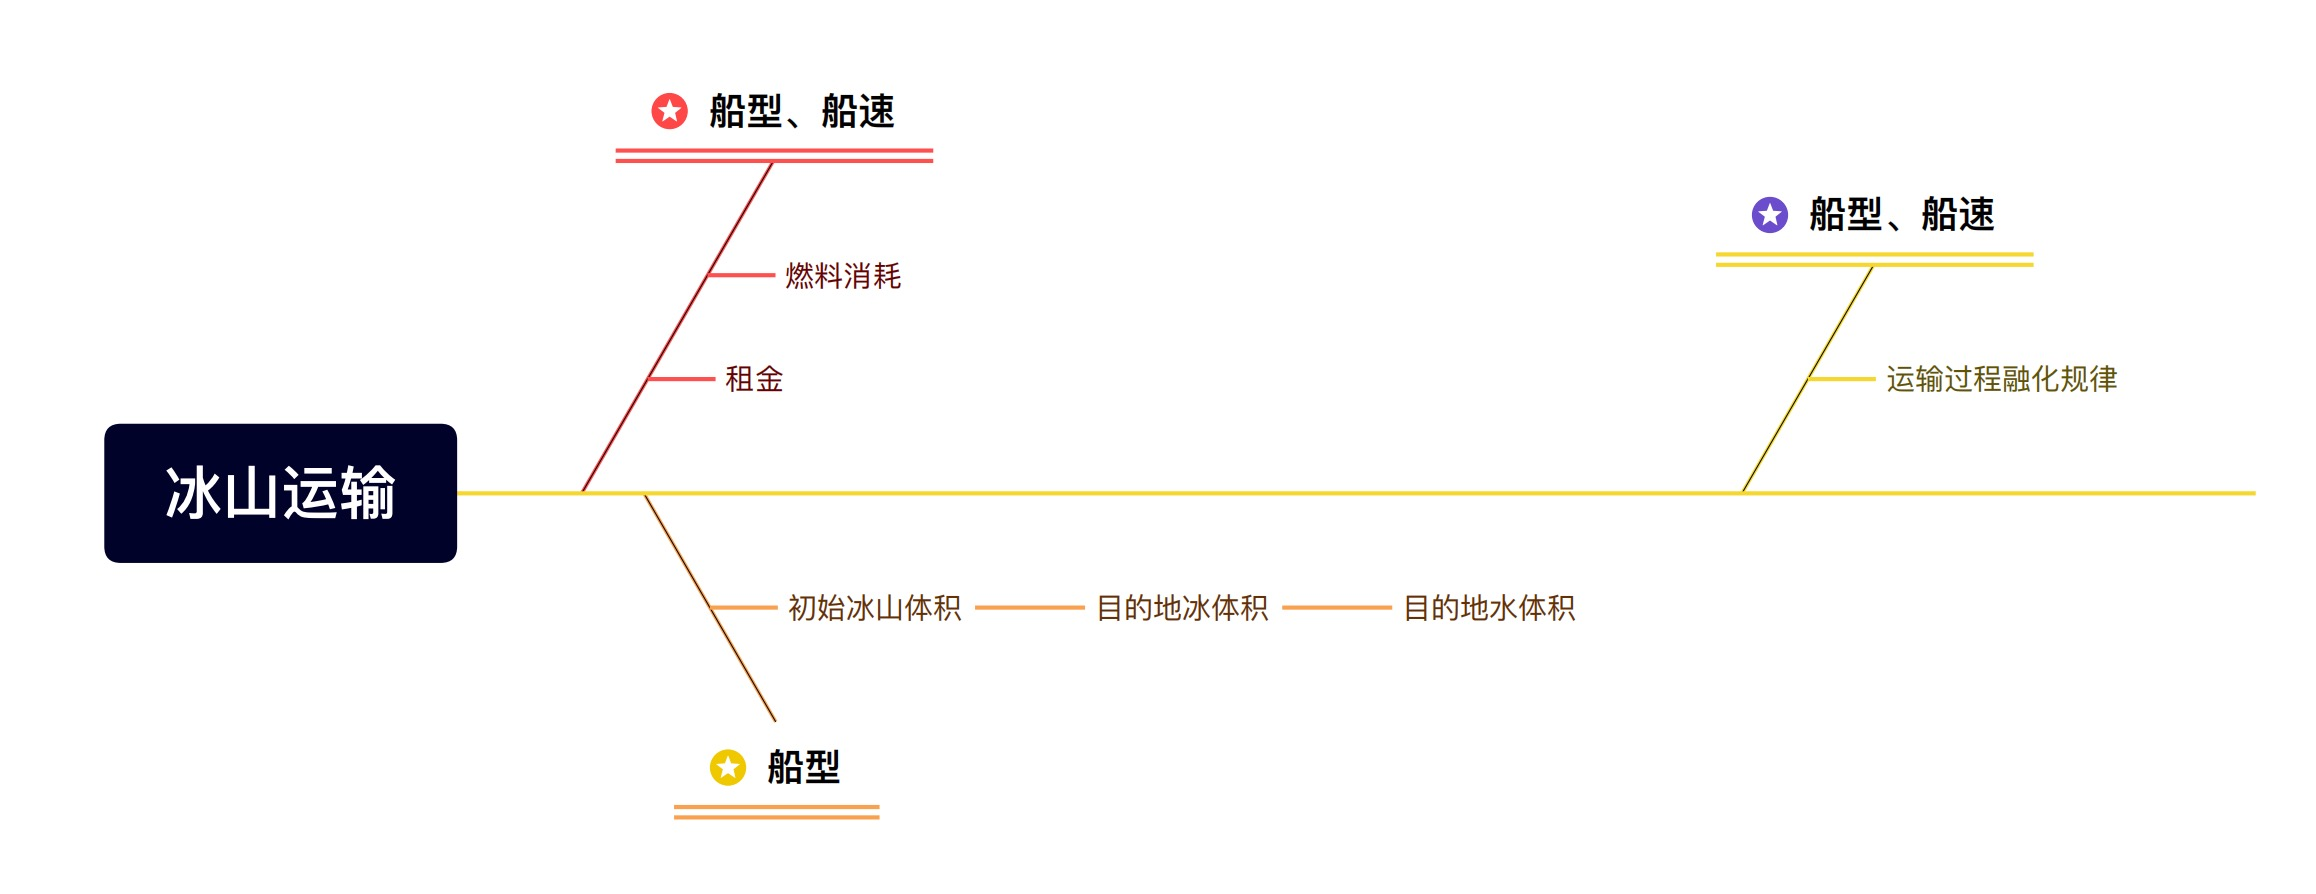
\includegraphics[scale=0.2]{wentifenxi.jpg}
\end{figure}
\section{模型假设}
\paragraph{(1)}拖船每天24小时不间断匀速前行,不考虑海啸、风暴等极端天气变化。
\paragraph{(2)}假定冰山为长方体。考虑到空气的导热系数大大低于水的导热系数,且冰山浮于海洋表面的部分相对整体较小,故不讨论冰山水上部分的融化情况。对于水下部分,认为每一点的融化速率是相同的。
\paragraph{(3)}考虑到从南极边缘地带到达波斯湾跨越了两个温度带,粗略地将行程前半段归为南温带,后半段归为热带,这直接影响了对水温的估计。
\paragraph{(4)}由于行程过长,为简化计算,将拖船与冰川看作一个质点,且不考虑洋流速度对该质点航行产生的影响,即认为全程的海面是几乎静止的。
\paragraph{(5)}查询相关资料得知,波斯湾平均深度30米,最深约100米。而冰山的水下部分需至少50米以保证运行过程中的稳定性。考虑到冰山的形状可以人为选择和切割,综合冰水密度比,为计算方便,假定冰山的水下部分固定为54米,水上部分固定为6米,即所有长方体冰山的竖直长度均为60米。而根据实际经验及一些真实冰山运输图片,假定长方体冰山的长宽之比为2:1.
\begin{figure}[H]
	\centering
	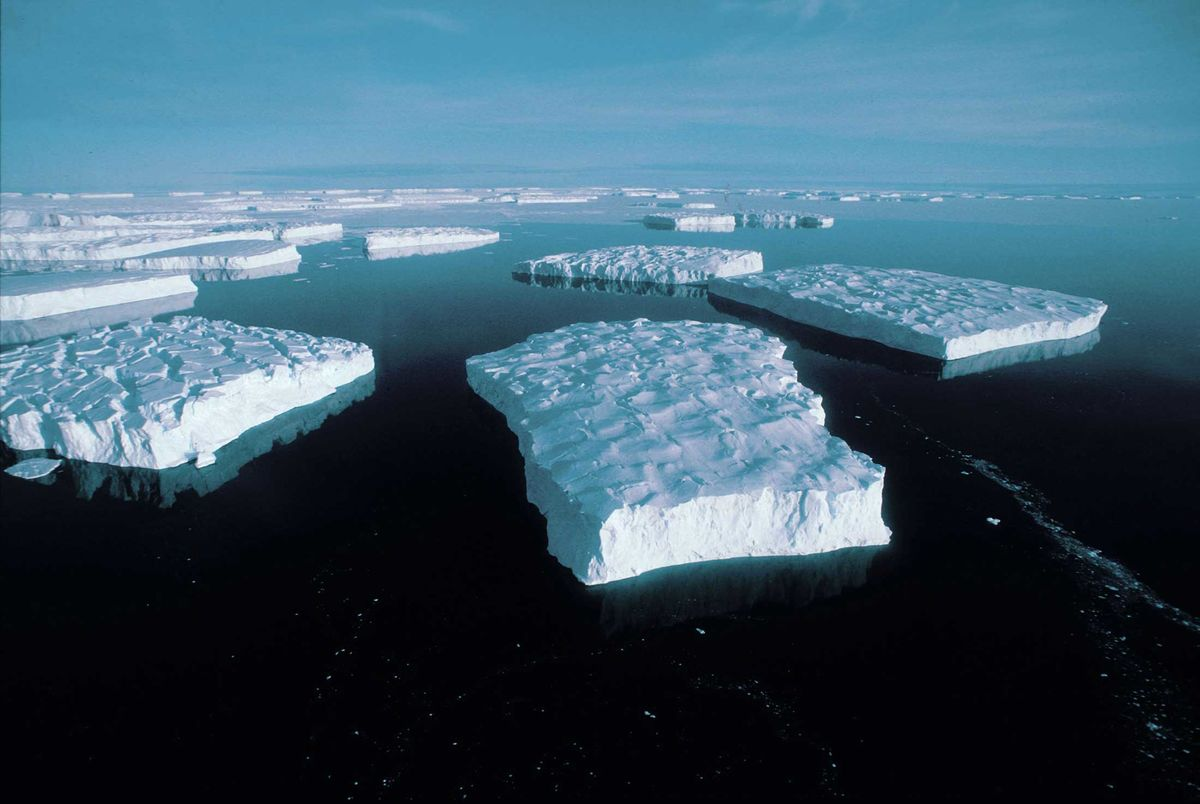
\includegraphics[scale=0.26]{res2/Iceberg.jpg}
	\caption{用于运输的冰山}
\end{figure} 
%\section{符号说明}
%\begin{table}[H]
%	\centering
%	\setlength{\abovecaptionskip}{0pt}%    
%	\setlength{\belowcaptionskip}{5pt}%
%	\setlength{\tabcolsep}{16mm}
%	\caption{符号说明}\label{y}
%	\begin{tabular}{cc}
%		\toprule
%		符号 & 说明                                        \\ \midrule
%		$R_{t}$     & 第$t$天的时变再生数             \\
%		$r$         & 确诊病例数             \\
%		$\lambda$     	& 平均感染率           \\
%%		$p$    & 原假设显著性检验中拒绝零假设的最低显著性水平\\
%		$T_{dp}$     & 露点温度             \\
%		$T$     & 干球温度             \\
%		$RH$     & 相对湿度             \\\midrule
%	\end{tabular}
%\end{table}
\section{模型建立}
对一选定的冰山,设其初始体积为$V_{0}$,则根据假设\textbf{(5)},其位于水下的体积为 $0.9~V_{0}$,我们仅讨论水下部分的融化情况。查询相关资料得知,南温带的平均海水温度约为 10 摄氏度,而热带的平均海水温度约为 20 摄氏度。
\subsection{冰山的体积变化}
为了计算冰山的融化速率,我们需要计算传热系数。考虑到冰山的体积庞大,其表面可以视作无穷大,在这个条件下进行简化处理后得到的平均传热系数用 $\alpha$ 表示,其计算公式为
\begin{equation}
	\alpha = Bw_{g}
\end{equation}
其中$w_{g}$表示冰山的运行速度。$B$ 为一比例系数,由公式
\begin{equation}
	B=0.00626~\frac{\lambda}{v}
\end{equation}
给出。其中 $\lambda$ 为水在 0 摄氏度时的导热系数,值为 0.551,单位为 W/m·K;$v$ 为同温度下水的运动黏度,值为$1.78\times10^{-6}$,单位为m$^{2}$/s. 公式(1)表明,在运行速度和温度不发生太大变化的情况下,冰山与水的传热系数与冰山的运行速度线性相关。而根据参考文献,冰山的融化速率 $w_{l}$(单位:m/1000s)可由以下公式计算
\begin{equation}
	w_{l}=\frac{\alpha(T_{w}-T_{l})}{r\rho_{l}}
\end{equation}
其中,$T_{w}$ 表示水温,$T_{l}$ 表示冰表面的温度,认为是 0 摄氏度。$r$ 为冰融化需要吸收的热量,一般取 334 kJ/kg. $\rho_{l}$ 为水下部分冰的密度,取 917 kg/m$^{3}$. 考虑到一天为 86400 秒,故水下部分的融化速率可表示为为 $8.64~w_{l}$ m/天。\par
接下来讨论在固定的 $w_{l}$ 下,冰川融化后的体积 $V\prime$。设时间 $\tau$(单位:天),则对于水下冰面上的任意一点,其融化深度为 $wt$. 根据参考文献\cite{filin2021multi},在已知水下高度 $h$(由假设,为54m)的情况下,长度 $2a$,宽度 $a$ 可由体积公式计算得出:
\begin{equation}
		a=\sqrt{\frac{V_{0}}{120}}
\end{equation}
由几何知识,水下部分融化后剩余体积为
\begin{equation}
	V(\tau)= (a-2\times8.14~w_{l}\tau)(2a-2\times8.14~w_{l}\tau)(h-8.14~w_{l}\tau)
\end{equation}
考虑到水面上部分的体积,融化后体积的计算公式为:
\begin{equation}
	V\prime=1.11V(\tau)
\end{equation}

\subsection{燃料消耗的费用}
以 $q_{fuel}$ 计燃料消耗费用率,单位为英镑/km. 观察表 2可知,当船速 $w_{g}$ 和体积的对数 $\text{lg}V$ 其中之一固定时,$q_{fuel}$ 是另一个变量的线性函数。因此不妨设
\begin{equation}
	q_{fuel}=c_{1}(w_{g}+c_{2})(\text{lg}V+c_{3})
\end{equation}
其中 $c_{1},c_{2},c_{3}$ 为待定系数。代入表 2 中数据求解,得$c_{1}=0.3,c_{2}=6,c_{3}=-1$. 对于固定的船速 $w_{g}$,当过去的天数为$\tau$ 时,燃料消耗总费用可由积分
\begin{equation}
	\begin{aligned}
	Q_{fuel}&=\int_{0}^{\tau}q_{fuel}d(24w_{g}\tau)\\
	&=\int_{0}^{\tau}0.3~(w_{g}+6)(\text{lg}V\prime-1)d(24w_{g}\tau)\\
	&=7.2~w_{g}(w_{g}+6)\int_{0}^{\tau}(\text{lg}V\prime-1)~d(\tau)
	\end{aligned}
\end{equation}
\subsection{总费用}
拖船的总天数 $t$ 由船速 $w_{g}$ 决定,为 $$t=\frac{9600}{24w_{g}}=\frac{400}{w_{g}}$$而拖船的日租金与最大运量有关,即与冰山的初始体积$V_{0}$有关,记作$f(V_{0})$. 故租船的费用为$$Q_{chater}=~f(V_{0})\frac{400}{w_{g}}$$.
综合以上信息可得,总费用为
\begin{equation}
	\begin{aligned}
	Q_{total}&=Q_{fuel}+Q_{chater}\\
	&=7.2~w_{g}(w_{g}+6)\int_{0}^{\frac{400}{w_{g}}}~(\text{lg}V\prime-1)~d(\tau)+~f(V_{0})\frac{400}{w_{g}}
	\end{aligned}
\end{equation}
\subsection{每立方米水需要的费用}
由给出信息,每立方米冰可融化为0.85立方米水。故获得的每立方米水的费用为
\begin{equation}
	\begin{aligned}
	\bar{Q}&=\frac{Q_{total}}{0.85V\prime}\\
	&=\frac{7.2~w_{g}(w_{g}+6)\int_{0}^{\frac{400}{w_{g}}}~(\text{lg}V\prime-1)~d(\tau)+~f(V_{0})\frac{400}{w_{g}}}{0.85V\prime}
	\end{aligned}
\end{equation}
\section{模型求解}
使用MATLAB软件进行求解,根据生活经验,仅计算船速为3-5km/h,冰山体积为$10^{6}-10^{7}m^{3}$的情况,计算过程见附录。得到结果如表所示。
\begin{table}[H]
	\centering
	\caption{求解结果}
	\begin{tabular}{c|ccc} 
		\hline
		\diagbox{船速(km/h)}{运量($m^{3}$)}                      & $10^{6}$      & $5\times10^{6}$     & $10^{7}$       \\ 
		\hline
		 3                      & 3.3094 & 0.2056 & 0.0889  \\
	  	 4 & 3.7006 & 0.2280 & 0.0986  \\
		 5                          & 4.0648 & 0.2505 & 0.1083  \\
		\hline
	\end{tabular}
\end{table}
由表可见,选择运量为$10^{7}m^{3}$的大船,船速为3km/h时,获取每立方米水的成本最低,为0.0889英镑,为直接蒸发海水成本的88.9\%,故在经济角度是可行的。
\section{模型评价}
相较于球形冰山模型,我们对冰山作出的假设更加合理,且考虑了水上水下融化速率不同的事实。然而我们建立的模型没有考虑洋流影响,根据参考文献\cite{filin2021multi},洋流的速度可达1-2千米每时,相较于本题中的船速并非可以忽略。即使不考虑大风浪等对拖船行驶造成困难的情况,洋流速度也会对燃料消耗造成较大的影响,这会导致实际情况与模型的较大差异。


\addcontentsline{toc}{section}{References}
	\bibliographystyle{IEEEtran}
	\bibliography{cite2}
	
\section*{附录:模型求解}\addcontentsline{toc}{section}{附录:模型求解}
\begin{lstlisting}[language=MATLAB]
clear;clc;
wg=[3,4,5];
Tw=[10,20];
V0=[1000000,5000000,10000000];
answer=zeros(3,3);
answerint=zeros(3,3);
Vprime=zeros(3,3);
fv0=0;
for i=1:3
for j=1:3
a=sqrt(V0(j)/120);
t=400/wg(i);
wl1=0.006*wg(i)*Tw(1);
Vtau=(a-2*3*wl1*0.5*t)*(2*a-2*3*wl1*0.5*t)*(54-3*wl1*0.5*t);
Vprime(i,j)=1.11*Vtau;
fun=@(t)7.2*wg(i)*(wg(i)+6)*log10(Vprime(i,j))-1+0*t;
answerint(i,j)=integral(fun,0,t);
if V0(j)<500000
fv0=4;
elseif (500000<V0(j))&&(V0(j)<1000000)
fv0=6.2;
elseif V0(j)>1000000
fv0=8;
end
answer(i,j)=(answerint(i,j)+fv0*t)/(0.85*Vprime(i,j));
end
end

\end{lstlisting}
\end{document}
